\documentclass[12pt]{article}
\usepackage[margin=1in]{geometry}
\usepackage{amsmath}
\usepackage{amssymb}
\usepackage{tikz}
\usepackage{pgfplots}
\usepackage{eso-pic}
\pgfplotsset{compat=1.18}

\AddToShipoutPictureBG{%
  \begin{tikzpicture}[remember picture,overlay]
    \foreach \y in {0,1,...,27} {
      \draw[gray!20, very thin] 
        ([yshift=-\y cm]current page.north west) -- 
        ([yshift=-\y cm]current page.north east);
    }
  \end{tikzpicture}
}

\setlength{\parindent}{0pt}
\setlength{\parskip}{8pt}

\title{Week 8: Short Review Test\\Weeks 1--7 Concepts}
\author{
	Student: SA\\
	Tutor: Rachel Eglash}
\date{November 5, 2025}

\begin{document}
	
	\maketitle

	\section*{Instructions}
        
        \begin{itemize}
            \item Show all work for full credit
            \item Circle your final answers
            \item No calculators
        \end{itemize}
	    
        \newpage
	
        \section*{Part A: Foundations \& Equations}

            \textbf{Problem 1}\\\\
            Simplify: $6 + 15 \div 3 - 2 \times 4$

            \vspace{3cm}

            \textbf{Problem 2}\\\\
            Simplify: $5(3x - 2) = - 2(x + 4)$

            \vspace{3cm}

            \textbf{Problem 3}\\\\
            Solve for $W$: $\displaystyle P = 2L + 2W$

            \newpage

        \section*{Part B: Inequalities}

            \textbf{Problem 4}\\\\
            Solve and graph: $-3x + 5 \leq -4$

            \vspace{3cm}

            \begin{center}
            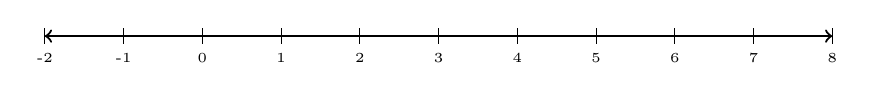
\begin{tikzpicture}
                \draw[<->,thick] (-2,0) -- (8,0);
                \foreach \x in {-2,-1,0,1,2,3,4,5,6,7,8}
                    \draw (\x,0.1) -- (\x,-0.1) node[below] {\tiny\x};
            \end{tikzpicture}
            \end{center}

            \vspace{1cm}

            Write in interval notation: \underline{\hspace{4cm}}

            \vspace{2cm}

            \textbf{Problem 5}\\\\
            Solve: $|2x - 3| < 7$

            \vspace{4cm}

            Write in interval notation: \underline{\hspace{4cm}}

            \newpage

        \section*{Part C: Linear Functions \& Lines}

            \textbf{Problem 6}\\\\
            Find the slope of the line through $(2, 5)$ and $(6, -3)$.

            \vspace{3cm}

            \textbf{Problem 7}\\\\
            Write the equation of a line with slope $\displaystyle\frac{3}{4}$ and y-intercept $-2$.

            \vspace{3cm}

            \textbf{Problem 8}\\\\
            Find the equation of the line through $(3, -1)$ and perpendicular to $y = -2x + 5$.

            \newpage

        \section*{Part D: Systems of Equations}

            \textbf{Problem 9}\\\\
            Solve the system:
            \begin{align*}
                y &= 3x - 4\\
                y &= -x + 8
            \end{align*}

            \newpage

        \section*{Part E: Applications}

            \textbf{Problem 10}\\\\
            A gym membership costs \$50 per month plus a one-time \$100 registration fee.\\\\
            Write an equation for the total cost $C$ after $m$ months.\\\\

            \vspace{2cm}

            Find the total cost after 6 months.

            \vspace{3cm}

            \textbf{Problem 11}\\\\
            A store sells notebooks and pens.\\\\
            There were 80 items sold in total.\\\\
            Notebooks cost \$3 each and pens cost \$2 each.\\\\
            The total revenue was \$190.\\\\
            How many notebooks were sold?

            \newpage

            \textbf{Problem 12}\\\\
            Two cars leave from the same location at the same time, traveling in opposite directions.\\\\
            Car A travels at 55 mph and Car B travels at 65 mph.\\\\
            After how many hours will they be 300 miles apart?

            \newpage

    \section*{Answer Key}

        \textbf{Problem 1}\\
        $6 + 15 \div 3 - 2 \times 4 = 6 + 5 - 8 = 3$\\

        \textbf{Problem 2}\\
        \begin{align*}
        5(3x - 2) &= -2(x + 4)\\
        15x - 10 &= -2x - 8\\
        17x &= 2\\
        x &= \frac{2}{17}
        \end{align*}\\

        \textbf{Problem 3}\\
        \begin{align*}
        P &= 2L + 2W\\
        P - 2L &= 2W\\
        W &= \frac{P - 2L}{2}
        \end{align*}\\

        \textbf{Problem 4}\\
        \begin{align*}
        -3x + 5 &\leq -4\\
        -3x &\leq -9\\
        x &\geq 3
        \end{align*}
        Interval notation: $[3, \infty)$\\
        Graph: Closed circle at 3, arrow pointing right\\

        \textbf{Problem 5}\\
        \begin{align*}
        |2x - 3| &< 7\\
        -7 < 2x - 3 &< 7\\
        -4 < 2x &< 10\\
        -2 < x &< 5
        \end{align*}
        Interval notation: $(-2, 5)$\\

        \newpage

        \textbf{Problem 6}\\
        $m = \displaystyle\frac{y_2 - y_1}{x_2 - x_1} = \frac{-3 - 5}{6 - 2} = \frac{-8}{4} = -2$\\

        \textbf{Problem 7}\\
        $y = \displaystyle\frac{3}{4}x - 2$\\

        \textbf{Problem 8}\\
        Perpendicular slope: $\displaystyle\frac{1}{2}$\\
        Using point-slope form:
        \begin{align*}
        y - (-1) &= \frac{1}{2}(x - 3)\\
        y + 1 &= \frac{1}{2}x - \frac{3}{2}\\
        y &= \frac{1}{2}x - \frac{5}{2}
        \end{align*}\\

        \textbf{Problem 9}\\
        \begin{align*}
        3x - 4 &= -x + 8\\
        4x &= 12\\
        x &= 3
        \end{align*}
        $y = 3(3) - 4 = 5$\\
        Solution: $(3, 5)$\\

        \textbf{Problem 10}\\
        Equation: $C = 100 + 50m$\\
        After 6 months: $C = 100 + 50(6) = 100 + 300 = \$400$\\

        \textbf{Problem 11}\\
        Let $n$ = notebooks, $p$ = pens\\
        $n + p = 80$\\
        $3n + 2p = 190$\\
        From first equation: $p = 80 - n$\\
        Substitute: $3n + 2(80 - n) = 190$\\
        $3n + 160 - 2n = 190$\\
        $n = 30$\\
        Answer: 30 notebooks\\

        \textbf{Problem 12}\\
        Combined speed: $55 + 65 = 120$ mph\\
        Distance = Rate $\times$ Time\\
        $300 = 120t$\\
        $t = 2.5$ hours

\end{document}